\chapter{Stand der Technik}\label{chap:sdt}

In diesem Kapitel wird in \hyperref[sec:InceptionTime]{Abschnitt 4.1} zunächst eine Übersicht über aktuelle Ansätze in der Zeitreihenklassifikation gegeben. Anschließend werden in \hyperref[sec:DLEKG]{Abschnitt 4.2} Ansätze zur Klassifikation von \gls{VHF} mittels \gls{DL} zusammengefasst. Zuletzt werden in \hyperref[sec:DGEKG]{Abschnitt 4.3} Vorgehen und die Ergebnisse einer systematischen Literaturrecherche zur \gls{DG} in der \gls{EKG}-Klassifikation präsentiert.

\section{Ansätze zur Zeitreihenklassifikation}\label{sec:InceptionTime}


Da \gls{EKG}-Daten Zeitreihendaten sind, muss für diese Arbeit eine \gls{DNN}-Architektur gewählt werden, die die zeitlichen Abhängigkeiten dieser Daten gut verarbeiten kann.
Fawaz et al. \cite{ismail_fawaz_deep_2019} haben in ihrem Review die gängisten Ansätze zur Zeitreihenklassifikation in einem einheitlichen Rahmen miteinander verglichen. Dazu wurden die gewählten Modelle auf insgesamt 97 uni- und multivariaten Zeitreihendatensätzen trainiert. Die 85 univariaten Zeitreihendatensätze stammen aus dem \textit{\gls{UCR}\slash\gls{UEA} time series archive} \cite{dau_ucr_2019} \cite{bagnall_great_2017}, die 12 multivariaten Datensätze stammen aus \textit{Baydogan's archive} \cite{baydogan_symbolic_2022}, welches 2015 auf der Website heruntergeladen werden konnte, aktuell jedoch nicht. Für univariate Zeitreihendaten, welche in dieser Arbeit als Ein-Kanal-\gls{EKG}s zu finden sind, zeigte beim paarweisen Vergleich von neun \gls{DNN}-Klassifikatoren das \gls{ResNet} die höchste Klassifikationsgüte. Dies ist dargestellt im Critical Difference Diagramm in \hyperref[fig:CritDiffReview]{Abb.~4.1}. Je niedriger der Rang im Diagramm, desto höher ist die durchschnittliche Klassifikationsgüte des Modells. Mit einer Querlinie verbundene Modelle unterscheiden sich statistisch nicht signifikant in ihrer Klassifikationsgüte. Zu sehen ist, dass das \gls{ResNet} einen Score von 2 besitzt und sich somit signifikant von den übrigen Modellen abhebt. Fawaz et al. veröffentlichten das im Rahmen des Reviews entwickelte Framework inklusive der implementierten Klassifikatoren\footnote{https://github.com/hfawaz/dl-4-tsc}. \cite{ismail_fawaz_deep_2019}

Nachträglich wurde von Fawaz et al. eine Website \cite{ali_ismail_fawaz_deep_nodate} erstellt, die eine Übersicht über die Ergebnisse des Vergleichsframeworks der im Review genutzten Klassifkatoren sowie neuerer Ansätze bietet. Ein neuerer Ansatz ist \textit{InceptionTime}, der eine bessere Leistung bezüglich Accuracy erzielt als ein \gls{ResNet}. Zu sehen in \hyperref[fig:CritDiff2]{Abb.~4.2} ist außerdem H-InceptionTime, welches ein hybrider Ansatz ist. Da sich diese Arbeit mit reinen \gls{DL}-Ansätzen beschäftigt, wird H-InceptionTime nicht weiter berücksichtigt.

\begin{figure}[!ht]%
\centering
	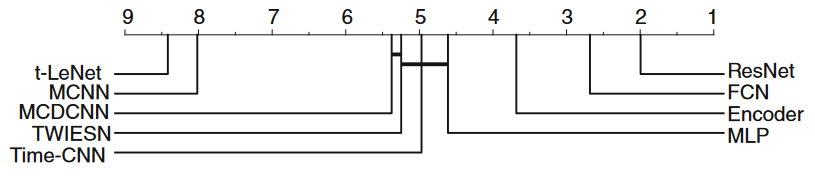
\includegraphics[width=0.80\textwidth]{./Bilder/crit_diff_review.png}
\caption[Critical Difference Diagramm aktueller Deep Neural Networks]{Das Critical Difference Diagramm zeigt die Klassifikationsgüte von neun Deep Neural Networks über das \gls{UCR}\slash\gls{UEA}-Archive im paarweisen Vergleich. Je niedriger der Rang, desto höher ist die durchschnittliche Klassifikationsgüte des Modells. Mit einer Querlinie verbundene Modelle unterscheiden sich statistisch nicht signifikant in ihrer Leistung. Entnommen aus \cite{ismail_fawaz_deep_2019}.} 
\label{fig:CritDiffReview}
\end{figure}  

\begin{figure}[!ht]%
\centering
	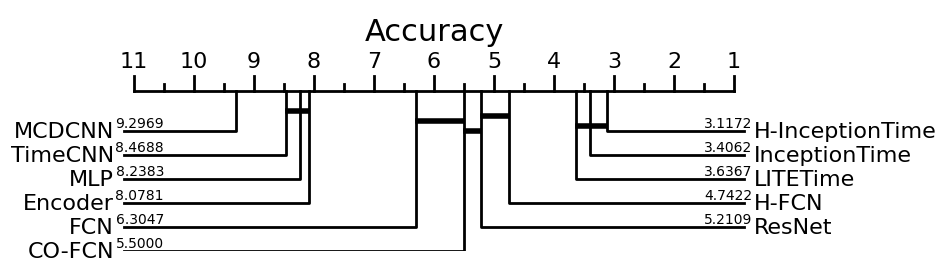
\includegraphics[width=0.80\textwidth]{./Bilder/crit_diff_acc.png}
\caption[Critical Difference Diagramm aktueller Deep Neural Networks und InceptionTime]{Das Critical Difference Diagramm zeigt die Klassifikationsgüte von Deep Neural Networks über das \gls{UCR}\slash\gls{UEA}-Archive im paarweisen Vergleich. Die Rangordnung der Klassifikatoren wurde basierend auf der Accuracy als Metrik erstellt. Je niedriger der Rang, desto höher ist die durchschnittliche Klassifikationsgüte des Modells. Mit einer Querlinie verbundene Modelle unterscheiden sich statistisch nicht signifikant in ihrer Leistung. Entnommen aus \cite{ali_ismail_fawaz_deep_nodate}.} 
\label{fig:CritDiff2}
\end{figure} 

InceptionTime \cite{fawaz_inceptiontime_2020} ist ein Ensemble aus \glspl{CNN} zur Zeitreihenklassifikation, welches auf Incep-tion-v4 basiert, einem \gls{CNN} zur Bildklassifikation. Als Eingabe können sowohl univariate als auch multivariate Zeitreihen dienen.  
Ein einzelner InceptionTime Klassifikator in der Standardkonfiguration ist aufgebaut aus zwei Residual Blocks, welche wiederum aus drei Inception Modulen gebildet werden. Es gibt, wie beim \gls{ResNet}, lineare Shortcut Verbindungen, die den Input des ersten Residual Blocks direkt zum Input des nächsten Residual Blocks hinzufügen. Auf die Residual Blocks folgt ein \gls{GAP} Layer, die den Durchschnitt der entstandenen multivariaten Zeitreihendaten über die gesamte Zeitdimension berechnet. Die letzte Schicht ist ein \gls{FC} Layer mit einer Softmax-Aktivierungsfunktion. Die Anzahl der Neuronen dieser Schicht entspricht der Anzahl der Klassen im Datensatz. In \hyperref[fig:InceptionTime]{Abb.~4.3} ist der Aufbau dargestellt. \cite{fawaz_inceptiontime_2020}

\begin{figure}[!ht]%
\centering
	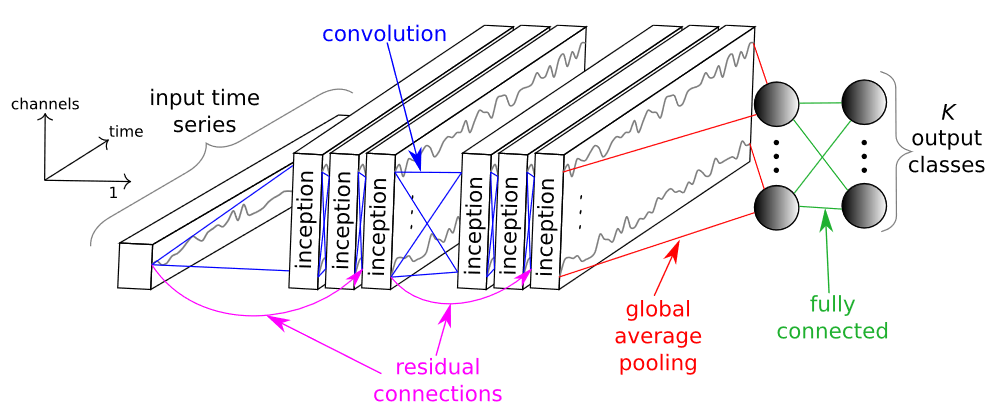
\includegraphics[width=1\textwidth]{./Bilder/InceptionTime.png}
\caption[Darstellung eines InceptionTime Klassifikators]{Darstellung eines einzelnen InceptionTime Klassifikators mit 6 Inception Modulen und einer univariaten Zeitreihe als Eingabe. Entnommen aus \cite{fawaz_inceptiontime_2020}.} 
\label{fig:InceptionTime}
\end{figure}  

In \hyperref[fig:InceptionModul]{Abb.~4.4} ist ein einzelnes Inception Modul dargestellt. Wird eine Zeitreihe der Dimension $M$ in ein Inception Modul eingegeben, so wird sie im ersten Schritt durch ein Bottleneck Layer mit $m$ Filtern mit Wahrnehmungsbereich und Schrittweite 1 auf eine Dimension von $m \ll M$ reduziert. Dies reduziert die Komplexität des Modells und somit auch das Overfitting, während gleichzeitig größere Filter als beim \gls{ResNet} ermöglicht werden. 
Im zweiten Schritt werden Convolutions mit verschieden großen Wahrnehmungsbereichen auf die Ausgabe des Bottleneck Layers angewandt. Parallel zu diesen Convolutions gibt es einen MaxPooling-Pfad, der die maximalen Werte innerhalb eines Fensters zusammenfasst und dadurch die Robustheit des Modells gegenüber Rauschen erhöht. Die Ausgabe der MaxPooling-Operation wird ebenfalls mittels eines Bottleneck Layers in ihrer Dimension reduziert. Die Ausgaben der unabhängigen Convolutions sowie der MaxPooling-Operation werden konkateniert und bilden die Ausgabe des Inception Moduls.
Die Standardkonfiguration eines Inception Moduls besteht aus 3 Filtersets mit jeweils 32 Filtern der Länge $l \in \{10, 20, 40\}$ und MaxPooling. Die Anzahl der Filter pro Schicht entspricht also $32 \times 4=128$. Die Größe des Bottleneck Layers liegt standardmäßig bei $m=32$. \cite{fawaz_inceptiontime_2020} 

Fawaz et al. empfehlen, InceptionTime als Ensemble zu verwenden, da es laut ihnen eine hohe Standardabweichung in der Accuracy zwischen einzelnen InceptionTime Klassifikatoren gibt. Ein InceptionTime Ensemble von Fawaz et al. besteht aus 5 unabhängig voneinander trainierten Modellen. Jedes Modell trägt mit demselben Gewicht zur finalen Vorhersage bei. Die Anzahl der einzelnen Modelle im Ensemble wurde bei 5 festgelegt, da keine signifikante Verbesserung bei mehr als 5 Modellen im Ensemble zu beobachten war.
Das InceptionTime Ensemble wurde mit einem \gls{ResNet} Ensemble der Größe 5 verglichen, da dies das bisher beste \gls{DL}-Ensemble für Zeitreihendaten war. Beide Ensembles wurden mit den 85 Zeitreihendatenbanken des UCR-Archives trainiert und evaluiert. In einem paarweisen Vergleich erzielte das InceptionTime Ensemble bessere Ergebnisse als das \gls{ResNet} Ensemble mit einem Win/Tie/Loss von 54/8/23. \cite{fawaz_inceptiontime_2020}

\begin{figure}[!ht]%
\centering
	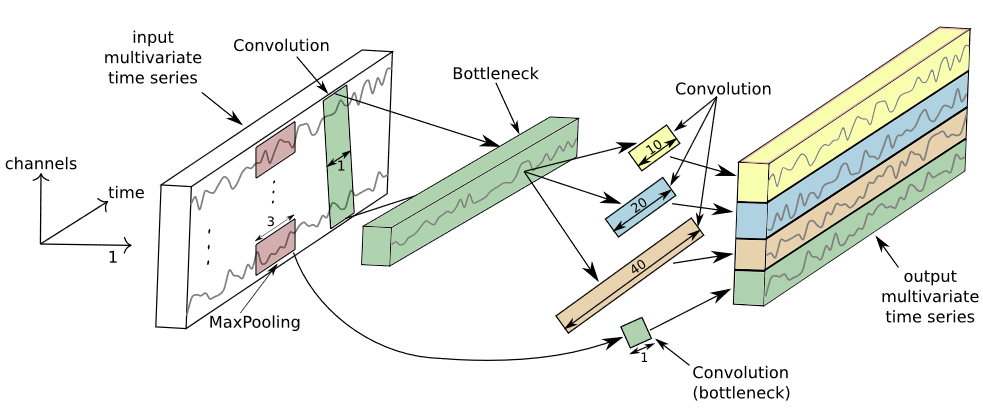
\includegraphics[width=1\textwidth]{./Bilder/InceptionModul.png}
\caption[Darstellung eines einzelnen Inception Moduls]{Darstellung eines einzelnen Inception Moduls mit einem Bottleneck Layer von $m=1$. Entnommen aus \cite{fawaz_inceptiontime_2020}.} 
\label{fig:InceptionModul}
\end{figure} 


%Default Hyperparameter: the default values for InceptionTime are: batch size 64; bottleneck size 32; depth 6; filter length {10,20,40}; and, number of filters 32.
 

\section{Ansätze zur Deep Learning-basierten Vorhofflimmern-Detektion in EKGs}\label{sec:DLEKG}

%full lead ecgs

%reduced lead ecgs
%Hier, das es möglich ist, VHF auf einer reduzierten kanalanzahl zu klassifizieren
%xECG Arch kann man hier auch mit erklären, dann ist das schonmal eingeführt

Es gibt bereits Ansätze zur erfolgreichen \gls{VHF}-Detektion in 12-Kanal-\gls{EKG}s mit Hilfe von \gls{DNN}s \cite{murat_et_al_review_2021}. Auch mit einer reduzierten Kanalanzahl kann \gls{VHF} erfolgreich mittels \gls{DNN}s detektiert werden \cite{murat_et_al_review_2021}. Ein Auszug an Ansätzen zu \gls{VHF}-Detektion sowohl mit voller als auch reduzierter Kanalanzahl ist in \hyperref[tab:DL_AF]{Tab.~4.1} zu sehen. Da in dieser Arbeit 10-Sekunden-\gls{EKG}s verwendet werden, wurden nur Ansätze ausgewählt, welche ebenfalls 10-Sekunden-\gls{EKG}s nutzen. Es werden F1-Scores von bis zu 0,991 mit 12-Kanal-\gls{EKG}s erreicht, sowie von bis zu 0,954 bei Nutzung eines Kanals.

\begin{table}[h!]
\centering
\caption[Deep Learning Ansätze zur VHF-Klassifikation]{Auswahl von Veröffentlichungen die Deep Learning zur Detektion von Vorhofflimmern mit 10-Sekunden-\gls{EKG}s nutzen. Wenn nur eine Ableitung genutzt wurde, wurde die genutzte Ableitung mit angegeben. Bei Lai et al. \cite{lai_non-standardized_2020} handelt es sich um einen Ein-Kanal-\gls{EKG}-Patch mit einer Platzierung, die mit Ableitung II korrespondiert.}
\label{tab:DL_AF}
\begin{tabular}{lllllll}
\hline
\textbf{\makecell{Referenz}} & \textbf{\makecell{Ableitungen}} & \textbf{\makecell{Algorithmus}} & \textbf{\makecell{Spec.}} & \textbf{\makecell{Rec.}} & \textbf{\makecell{Acc.}} & \textbf{\makecell{F1}}\\ \hline
 	\makecell{Attia et al., 2019 \cite{attia_artificial_2019}}	& \makecell{12} 	& \makecell{CNN} 	& \makecell{0,834}	& \makecell{0,823}	& \makecell{0,833} & \makecell{0,454} \\
 	
  	\makecell{Cai et al., 2020 \cite{cai_accurate_2020} }	& \makecell{12} 	& \makecell{DDNN} 	& \makecell{0,994}	& \makecell{0,992}	& \makecell{0,994} & \makecell{0,991}  \\
  	
  	\makecell{Ribeiro et al., 2020 \cite{ribeiro_automatic_2020} }	& \makecell{12} 	& \makecell{ResNet} 	& \makecell{1}	& \makecell{0,769}	& \makecell{-} & \makecell{0,870} \\ 
  	
 	\makecell{Lai et al., 2020 \cite{lai_non-standardized_2020} }	& \makecell{1 (modified II)} 	& \makecell{CNN} 	& \makecell{0,934}	& \makecell{0,931}	& \makecell{0,931} & \makecell{-} \\
 	
 	\makecell{Baalman et al., 2020 \cite{baalman_morphology_2020} }	& \makecell{1 (II)} 	& \makecell{RNN} 	& \makecell{-}	& \makecell{-}	& \makecell{0,960} & \makecell{0,940} \\ 	
 	
  	\makecell{Goettling et al., 2024 \cite{goettling_xecgarch_2024} }	& \makecell{1 (II)} 	& \makecell{CNN} 	& \makecell{0,958}	& \makecell{0,949}	& \makecell{0,953} & \makecell{0,954} \\
  				 		 		
\hline
\end{tabular}
\end{table}

\section{Verwendung von Domain Generalization in der EKG-Klassifikation}\label{sec:DGEKG}


\gls{DG} ist ein relevantes Problem in der \gls{EKG}-Klassifikation, da es eine Vielzahl an möglichen Domain Shifts gibt, jedoch in der Praxis selten bereits ein Testdatensatz während des Trainings vorliegt, um \gls{DAp}-Methoden wie Transfer Learning anzuwenden \cite{hasani_classification_2020}. Im Rahmen dieser Arbeit wurde eine systematische Literaturanalyse zur \gls{DG} in der \gls{EKG}-Klassifikation durchgeführt. Es wurden vier Suchstrings definiert (zu finden in \hyperref[sec:strings]{Anhang A.1}), mit welchen die Literaturdatenbanken \textit{IEEE Xplore}, \textit{PubMed} und \textit{Clarivate Web of Science} durchsucht wurden, resultierend in insgesamt 367 Suchergebnissen. Durch Titel- und Abstrakt-Screening wurden 39 relevante Veröffentlichungen gefunden. Nach dem Volltext-Screening dieser Veröffentlichungen wurden 7 als tatsächlich relevant identifiziert.    

Stammen Aufnahmen aus verschiedenen Krankenhäusern, tritt ein Domain Shift auf, da die \gls{EKG}s unter verschiedenen Bedingungen aufgenommen wurden \cite{hasani_classification_2020}. Ballas \& Diou \cite{ballas_domain_2022} \cite{ballas_towards_2024} beschäftigen sich mit diesem Domain Shift und entwickeln eine \gls{DL}-Architektur, welche auf ein \gls{ResNet}-18 aufsetzt und aus mittleren Convolutional Layern Merkmale extrahiert. Durch diese Extraktion aus mittleren Schichten soll die Verschmelzung von domäneninvarianten mit domänenspezifischen Merkmalen so gering wie möglich gehalten werden.

Hasani et al. \cite{hasani_classification_2020} verwenden als \gls{DG}-Methoden Data Augmentation und Domain Adversarial Learning. Dabei wurden bei der Datenvorverarbeitung zufällig Frequenzen aus den Aufnahmen herausgefiltert oder hinzugefügt, um die statistischen Eigenschaften der Trainingsdaten variabel zu gestalten. Zusätzlich wurden zufällig einzelne Ableitungen durch Nulllinien oder Rauschen ersetzt, Ableitungen vertauscht, Aufnahmen einzelner Ableitungen invertiert, ein Bandpass angewandt oder die Aufnahmen skaliert. Beim Training des Modells wurde ein Domain Adversarial Head mit einem \gls{GRL} und zwei \gls{FC}-Layer mit Dropout hinzugefügt, um die Generalisierung der Modelle über unbekannte Zieldomänen hinweg zu verbessern. Der Feature Extractor des Modells besteht aus zwei parallelen \gls{CNN}s mit unterschiedlich großen Wahrnehmungsbereichen, sodass sowohl grobe als auch feinere Merkmale extrahiert werden können. Auf die \gls{CNN}s folgen zwei \gls{LSTM} Layer, um zeitabhängige Merkmale zu extrahieren. Der Label Predictor besteht aus zwei \gls{FC}-Layern mit Dropout.

Shang et al. \cite{shang_deep_2021} entwickeln ebenfalls ein \gls{DANN} und nutzen als Domain die jeweilige Datenbank aus der die Aufnahmen stammen. Der Feature Extractor des \gls{DANN}s ist ein modifiziertes ResNet mit einem Convolutional Layer mit großen Wahrnehmungsbereich und 8 Residual Blocks. Der Domain Classifier besteht aus einem \gls{GRL} und drei \gls{FC}-Layern mit Dropout, wobei der Label Predictor aus zwei \gls{FC}-Layern ohne Dropout besteht.

Shin et al. \cite{shin_enhancing_2023} nennen ihre Methode zur \gls{DG} \glqq Denoise and Contrast Attention Module\grqq{}, welche auf ein U-Net aufsetzt. Im ersten Schritt werden die Aufnahmen mit Hilfe eines \gls{CNN}s entrauscht. Der Attention-Mechanismus analysiert im Anschluss die Unterschiede in der Morphologie und die zeitlichen Intervalle der Herzschläge, um ventrikuläre Extrasystolen zu detektieren.

Die bisher genannten Ansätze betrachten zwar den Domain Shift zwischen verschiedenen 12-Kanal-\gls{EKG}-Datenbanken, jedoch nicht den Domain Shift, der auftritt, wenn Signale morphologisch verändert sind. Solche Signale treten beim Domain Shift zwischen \gls{EKG}- und \gls{PPG}-Signalen oder zwischen 12-Kanal-\gls{EKG}- und \gls{EKG}-Patch-Signalen mit reduzierter Kanalanzahl auf.

Mit diesem Problem beschäftigen sich Shashikumar et al.~\cite{shashikumar_detection_2018} und Ramesh et al.~\cite{ramesh_atrial_2021}, indem sie Transfer Learning nutzen, um ihre auf \gls{EKG}s trainierten Modelle für \gls{PPG}-Signale anzupassen. Transfer Learning ist jedoch, wie bereits erwähnt, ein Ansatz aus der \gls{DAp} und setzt voraus, dass ein Trainingsdatensatz aus der Zieldomäne vorliegt. Shashikumar et al. \cite{shashikumar_detection_2018} extrahieren zeit-frequenzbezogene Merkmale aus den \gls{EKG}s und \gls{PPG}s und nutzen diese als Merkmale für ihren Klassifikator. 
Ramesh et al. \cite{ramesh_atrial_2021} nutzen nur Merkmale der \gls{HRV} zur \gls{VHF}-Klassifikation, da diese sowohl aus \gls{EKG}- als auch aus \gls{PPG}-Signalen extrahiert werden können. Sie evaluieren die Fähigkeit zur \gls{DG} ihres Modells sowohl mit als auch ohne Transfer Learning. Sowohl Shashikumar et al. \cite{shashikumar_detection_2018} als auch Ramesh et al.\cite{ramesh_atrial_2021} nutzen Ansätze, um auf morphologisch veränderten Signalen als Zieldomäne zu klassifizieren. Jedoch tun sie dies, indem sie Merkmale nutzen, in denen keine Informationen zur Signalmorphologie enthalten sind. In dieser Arbeit wird daher ein Ansatz verfolgt, der die Signalmorphologie berücksichtigt.

Eine Übersicht über verwendete Algorithmen, Methoden zur \gls{DG}, sowie Quell- und Zieldomänen ist in \hyperref[tab:tabelle_related]{Tab.~4.2} zu finden.

\begin{landscape}
\begin{table}[h!]
\centering
\caption[Deep Learning Ansätze zur DG in der EKG-Klassifikation]{Use Cases von Deep Learning Algorithmen zur Klassifikation von Elektrokardiogrammen (EKGs) mit Nutzung von Domain Generalization Methoden. Wenn möglich, wurde der F1-Score angegeben.
HRV: Herzratenvariabilität, PPG: Photoplethysmographie, VES: Ventrikuläre Extrasysolen, VHF: Vorhofflimmern}
\label{tab:tabelle_related}
\begin{tabular}{|l|l|l|l|l|l|l|}
\hline
\textbf{\makecell{Referenz}} & \textbf{\makecell{Algorithmus}} & \textbf{\makecell{Generalization\\Methode}} & \textbf{\makecell{Merkmale}} & \textbf{\makecell{Domänen}} & \textbf{\makecell{Performance\\Quelldomäne}} & \textbf{\makecell{Performance\\Zieldomäne}} \\ \hline

\makecell{Ballas \& Diou,\\ 2022 \cite{ballas_domain_2022}}		& \makecell{ResNet-18}	& \makecell{Feature\\ Disentanglement} & \makecell{Deep Features} & \makecell{12-Kanal-EKG-DBs\\ aus verschiedenen\\ Krankenhäusern} & \makecell{F1 0,94 (VHF)}  & \makecell{F1 0,91 (VHF)} \\ \hline

\makecell{Ballas \& Diou,\\ 2024 \cite{ballas_towards_2024}}		& \makecell{ResNet-18 \\ S-ResNet} & \makecell{Feature\\ Disentanglement} & \makecell{Deep Features} & \makecell{12-Kanal-EKG-DBs\\ aus verschiedenen\\ Krankenhäusern} & \makecell{ResNet-18\\ F1 0,88 (VHF)\\ S-ResNet\\ F1 0,87 (VHF)} & \makecell{ResNet-1\\ F1 0,64 (VHF)\\ S-ResNet\\ F1 0,63 (VHF)} \\ \hline

\makecell{Hasani et al.,\\ 2020 \cite{hasani_classification_2020}} 		& \makecell{CNN-LSTM} & \makecell{Data Augmentation,\\ Domain Adversarial\\ Learning} & \makecell{Alter, Geschlecht,\\ Deep Features} & \makecell{12-Kanal-EKG-DBs\\ aus verschiedenen\\ Krankenhäusern} & \makecell{CinC 2020 score \\ 0,63} & \makecell{CinC 2020 score \\ 0,44} \\ \hline

\makecell{Shang et al.,\\ 2021 \cite{shang_deep_2021} }			& \makecell{SE-ResNet} & \makecell{Domain Adversarial\\ Learning} & \makecell{Alter, Geschlecht,\\ HRV Features,\\ Deep Features} & \makecell{12-Kanal-EKG-DBs\\ aus verschiedenen\\ Krankenhäusern} & \makecell{CinC 2020 score\\ 12-Kanal 0,72\\ 6-Kanal 0,68} & \makecell{CinC 2020 score\\ 12-Kanal 0,44\\ 6-Kanal 0,49} \\ \hline

\makecell{Shin et al.,\\ 2023 \cite{shin_enhancing_2023}}			& \makecell{U-Net +\\ DCAM} & \makecell{Domain Invariant\\ Respresentation Learning\\ with Attention Model} & \makecell{Deep Features} & \makecell{12-Kanal-EKG-DBs\\ aus verschiedenen\\ Krankenhäusern} & \makecell{F1 0,99 (VES)} & \makecell{gemittelt über\\ 6 Zieldomänen\\F1 0,89 (VES)} \\ \hline

\makecell{Shashikumar\\ et al.,\\ 2018 \cite{shashikumar_detection_2018}}	& \makecell{CNN + BRNN +\\ Attention Model} & \makecell{Explicit Feature\\Alignment,\\Transfer Learning} & \makecell{Deep Features,\\ Time Series\\ Covariates,\\ Signal Quality\\ Indices} & \makecell{EKG, PPG} & \makecell{AUC 0,97} & \makecell{AUC 0,94} \\ \hline

\makecell{Ramesh et al.,\\ 2021 \cite{ramesh_atrial_2021}}			& \makecell{CNN} & \makecell{Explicit Feature\\ Alignment,\\ Transfer Learning} & \makecell{HRV Features} & \makecell{EKG, PPG} & \makecell{F1 0,93} & \makecell{Ohne\\ Transfer Learning\\F1 0,72\\Mit\\ Transfer Learning\\F1 0,89} \\ \hline

% &  &  &  &  &  &  \\ \hline
\end{tabular}
\end{table}
\end{landscape}